% !TeX root = ../../main.tex
\chapter{Implementation}
\label{chapter:scafi3-arch-reification}

This chapter discusses the incarnation of the proposed abstract architecture described in \Cref{chapter:contribution} to ScaFi3.
%
\todo{description of the flow}

\todo{project structure - shared, jvm-native, js-native, js, native, jvm and expect/actual Scala mechanism}

\section{High level architecture}

Building upon the ScaFi3 library architecture presented in \Cref{sec:scafi3-overview}, this work extends it to support distributed aggregate computing and polyglot capabilities as per the abstract architecture presented in \Cref{chapter:contribution}.
%
\begin{figure}
    \centering
    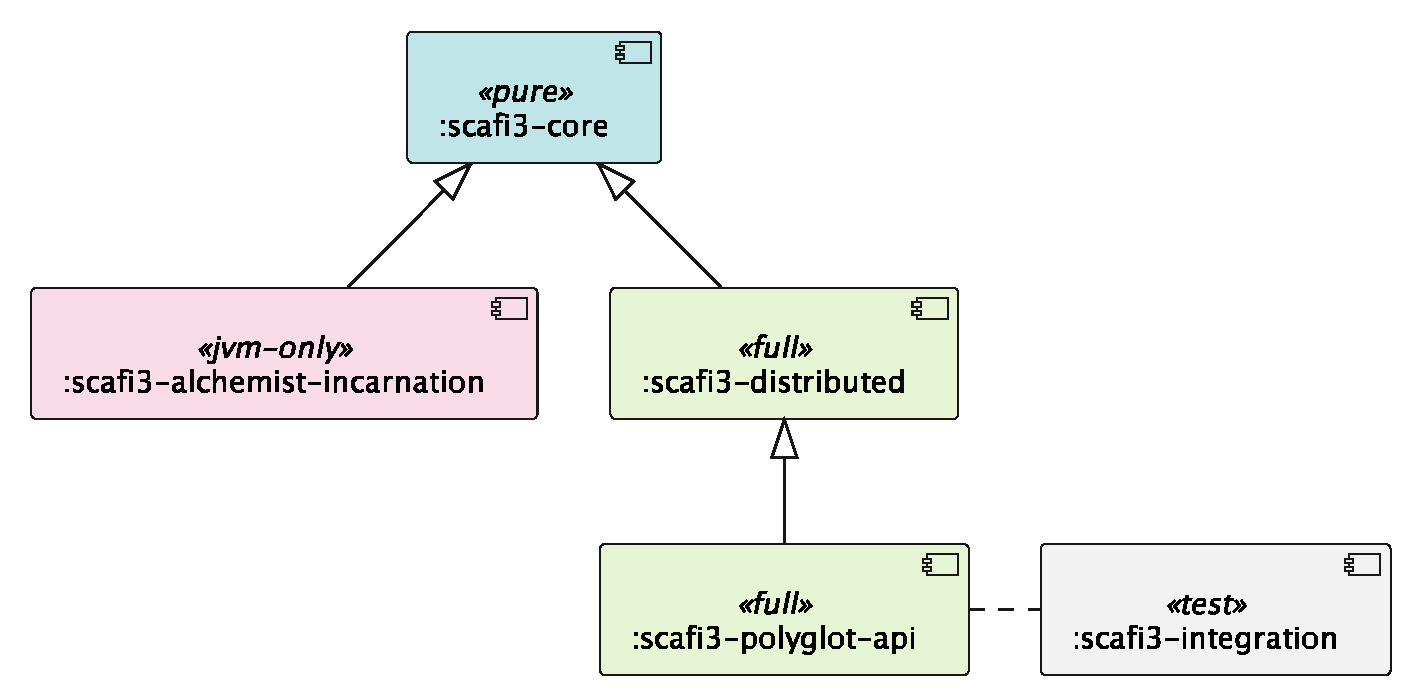
\includegraphics[width=0.7\textwidth]{resources/schemas/scafi3-architecture.eps}
    \caption{UML component diagram of the ScaFi3 architecture.}
    \label{fig:scafi3-architecture}
\end{figure}
%
The overall components and their dependencies are illustrated in \Cref{fig:scafi3-architecture} and comprise the following modules:
%
\begin{itemize}
    \item \textbf{Distribution module}: responsible for enabling distributed communication and messages exchange between devices, including the serialization and deserialization concerns;
    \item \textbf{Polyglot API module}: responsible for providing polyglot capabilities to the library;
    \item \textbf{Integration module}: where integration tests are performed to ensure the correct functioning of the polyglot and distributed capabilities of the library.
\end{itemize}

\section{Infrastructure module}

\subsection{Distribution module}

Enabling distribution in ScaFi3 requires implementing an abstract network manager that is able to send and receive Value Trees \todo{in context add Value Tree} from and to neighbor devices.
%
The AC framework abstract over the specific protocol used to communicate with neighbors and their discovery mechanism, allowing the implementation of different network managers for different protocols and scenarios.

As an initial step in ScaFi3's evolution toward full-featured distributed capabilities, a socket-based network manager has been implemented. 
%
This foundation layer employs stream, TCP-based connection-oriented sockets, intentionally prioritizing core communication reliability over advanced distributed features, which remain subjects for future work.
%
Indeed, despite the low-level nature of sockets, they provide a foundational abstraction layer that many higher-level protocols ultimately rely upon (such as HTTP, MQTT, etc.), making them a suitable starting point for building extensible communication mechanisms.
%
Consequently, as shown in \Cref{fig:socket-network-manager-architecture}, each device is bound to a specific endpoint (IP address and port) and communicates point-to-point with its neighbors.
%
\begin{figure}[h]
    \centering
    \includegraphics[width=\textwidth]{resources/img/socket-network-manager.pdf}
    \caption{Socket-based network manager high level architecture.}
    \label{fig:socket-network-manager-architecture}
\end{figure}

The UML class diagram of the socket-based network manager is shown in \Cref{fig:socket-network-manager-design}.
%
It adopts an asynchronous design leveraging Scala's Future-based API and comprises two primary active components that operate concurrently to handle bidirectional communication:
%
\begin{itemize}
    \item the incoming connection \texttt{Listener}, continuously listening for incoming messages from neighbor devices. Received messages are stored in a thread-safe \texttt{Map} that retains only the most recent message from each neighbor, according to a configurable \texttt{Retention Policy} that defines, in absence of new messages, how long a message should be retained before being discarded. The up-to-date view of all the received neighbor messages, a.k.a. their Value Trees, is made available to the ScaFi Engine through the \texttt{receive} method at the beginning of each round of computation;
    \item the outgoing message channel, providing a non-blocking interface for message transmission. Upon the end of each round of computation, the ScaFi Engine invokes the \texttt{send} method of the network manager to dispatch the device's current Value Tree to all its neighbors. For each neighbor, the corresponding Value Tree is pushed through the channel and, asynchronously, dispatched to the corresponding destination. To resolve neighbor addresses the socket-based network manager is mixed in with a \texttt{NeighborhoodResolver}, which provides the necessary endpoint resolution capabilities.
\end{itemize}
%
This dual component design ensure that both incoming and outgoing communications proceed without blocking, a pre-condition for targeting JavaScript environments and at the same time maintain system responsiveness.
%
\begin{figure}[h]
    \centering
    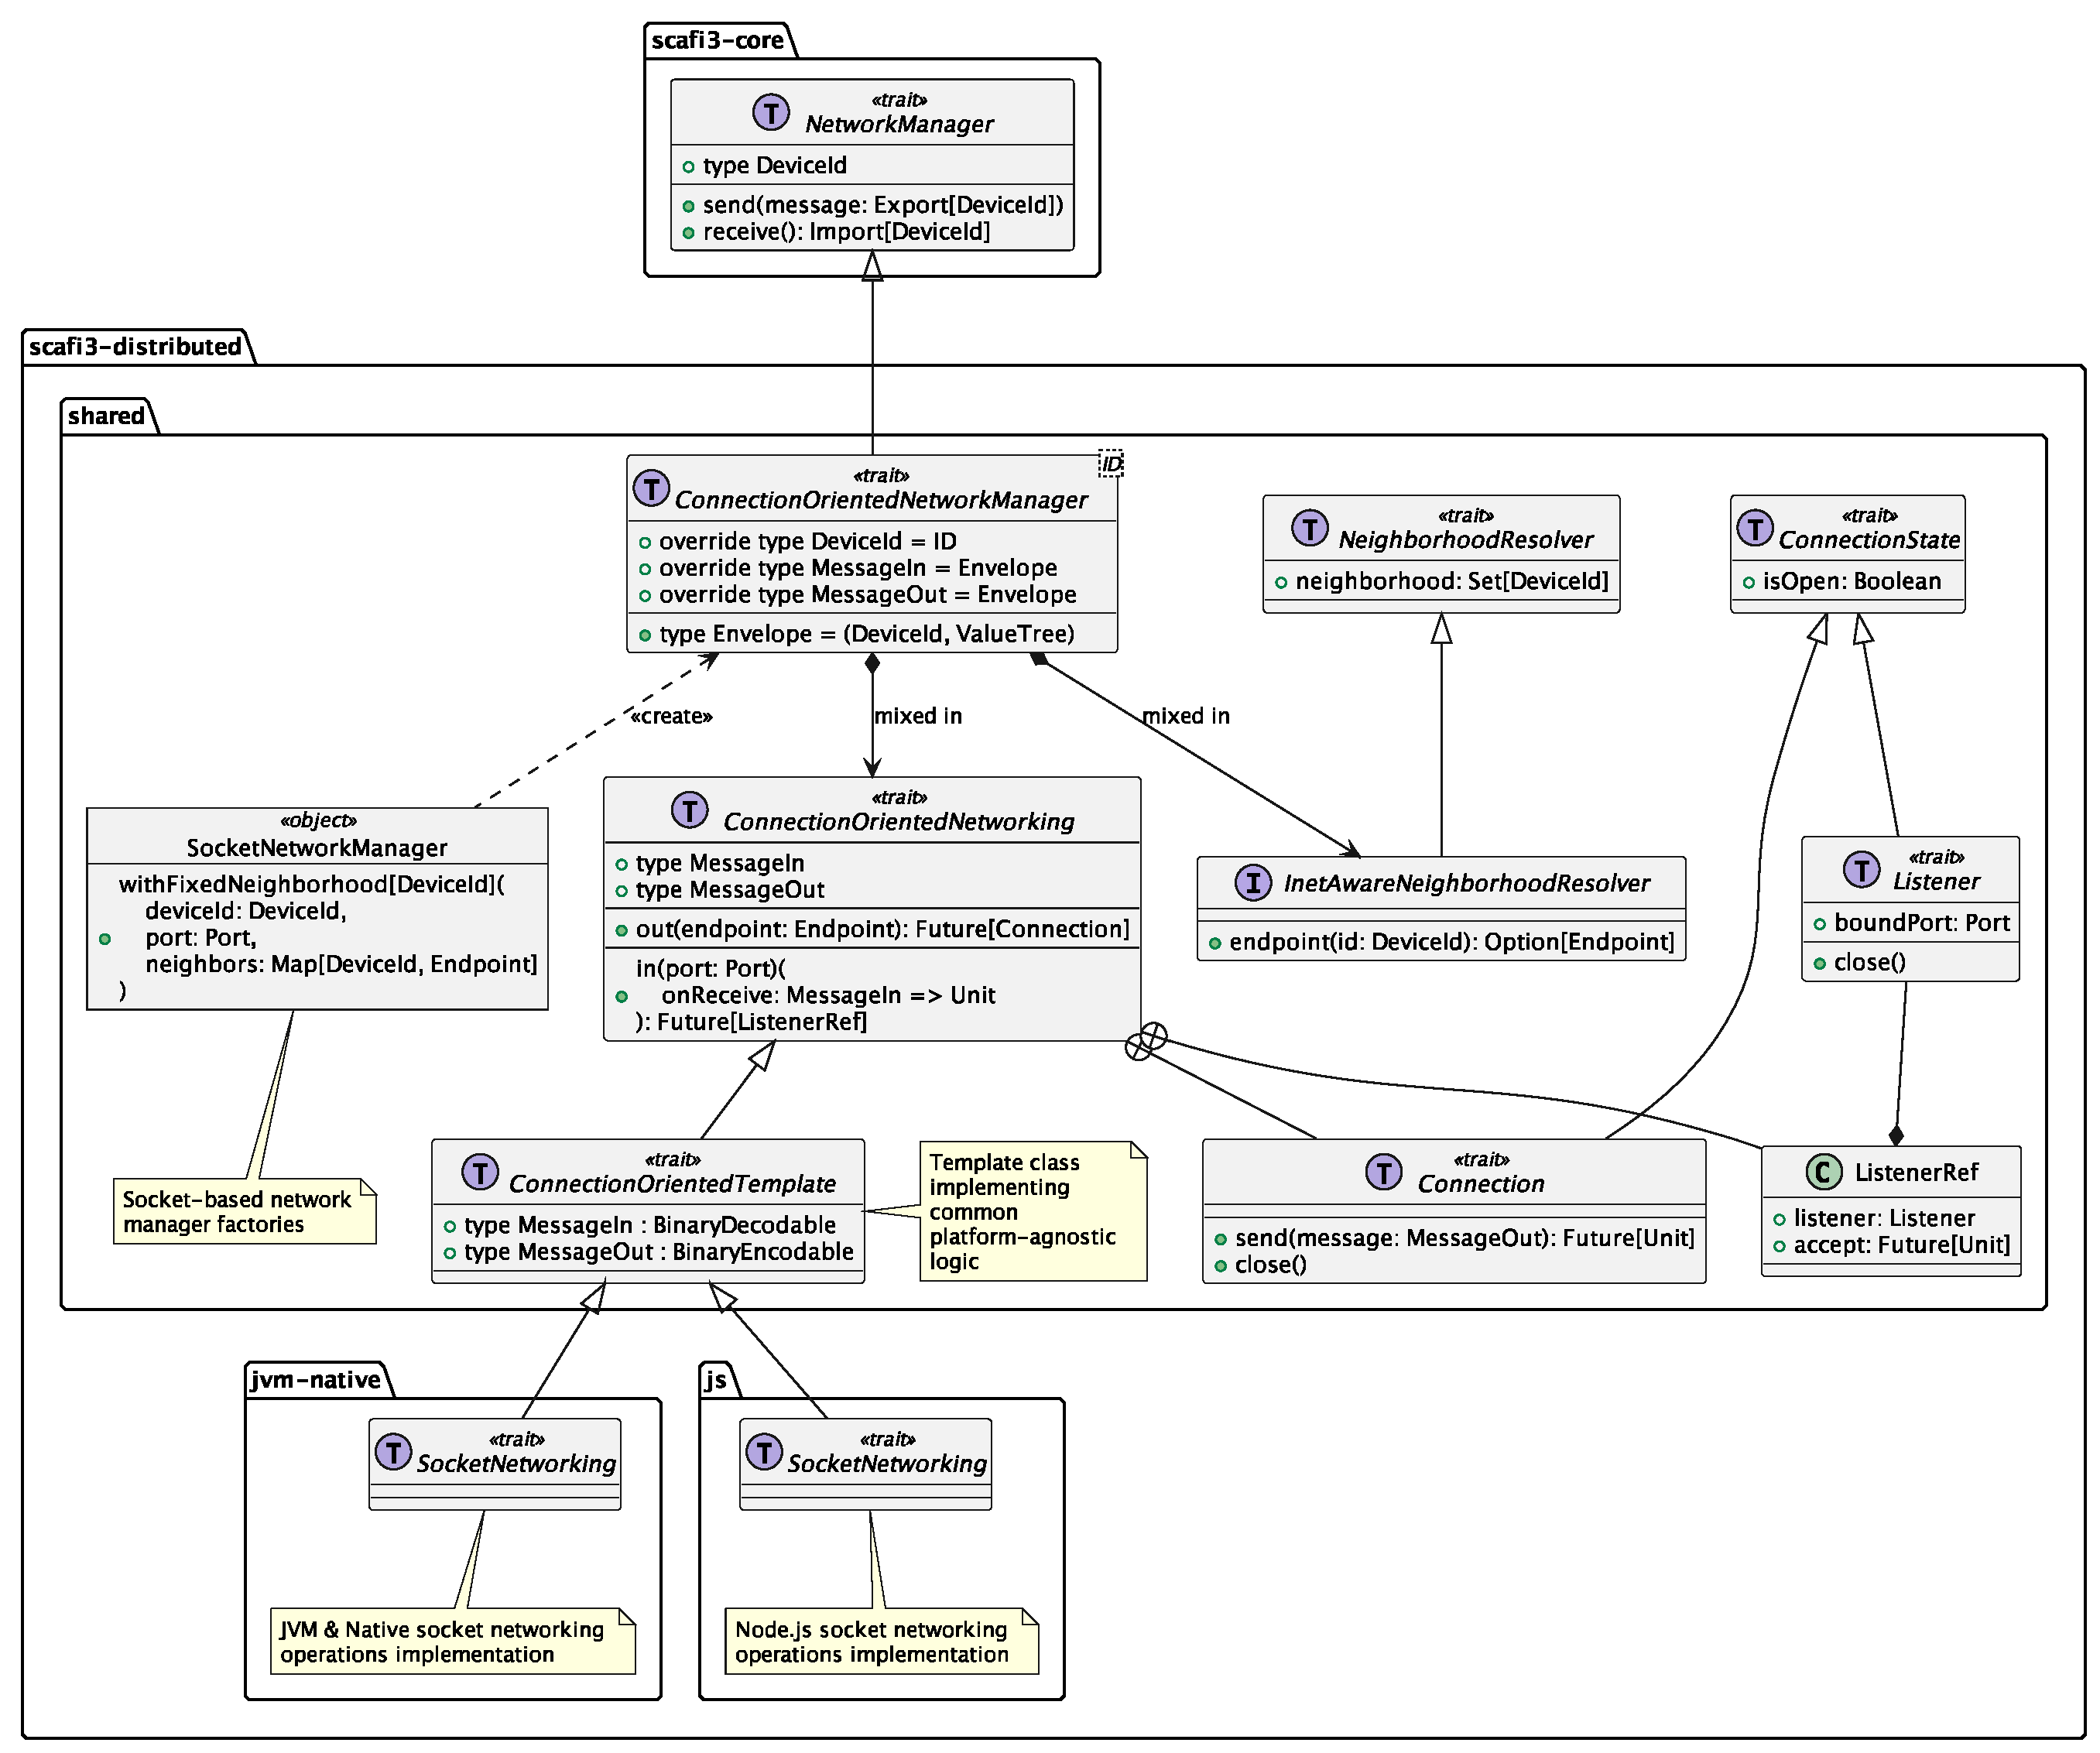
\includegraphics[width=\textwidth]{resources/schemas/socket-distribution.eps}
    \caption{UML diagram of the socket-based network manager design.}
    \label{fig:socket-network-manager-design}
\end{figure}

Remote socket-based communication logic are demanded to the \texttt{ConnectionOrientedNetworking} trait and their platform-specific implementations.
%
Since the absence of a cross-platform socket library supporting both client and server socket programming, two distinct implementations have been provided:
%
\begin{itemize}
    \item one for JVM and Native platforms, leveraging the \texttt{java.net} package available in the standard library. This has been made possible by Scala Native, which have reimplemented the \texttt{java.net} package to provide socket programming capabilities on native platforms. Programmers can thus use the same API on both JVM and Native platforms without any code divergence like they would do in pure Scala JVM applications;
    \item one for JavaScript platforms, leveraging the \texttt{Node.js} library API. For this, the \texttt{net} module of Node.js has been used, through a Scala.js facade that enables calling the Node.js API from Scala.js code. A portion of this facade is shown in \Cref{lst:js-sockets-facade}. This is essentialy the transposition of Node.js API definitions into Scala trait and classes using Scala.js types, annotations and placeholders that, when linked, allow Scala.js code to call the underlying Node.js API.
\end{itemize}

\lstinputlisting[
    language=Scala, 
    label={lst:js-sockets-facade},
    caption={Portion of the Scala.js facade for the Node.js \texttt{net} module.},
    linerange={46-54},
]{resources/code/JSSocketsFacade.scala}

Despite targeting all three platforms, the design differs only in platform-specific networking logic, isolated within respective \texttt{SocketNetworking} traits. 
%
This separation leverages Scala's mixin composition and the template method pattern, defining common logic in abstract trait (\texttt{ConnectionOrientedTemplate}) while deferring platform-specific details to specialized implementations.

\subsection{Serialization binding}

Another essential requirement is the provision of serialization and deserialization capabilities for message exchange between devices.

Since ScaFi3 devices exchange pairs of Device Identifiers and their corresponding Value Trees, serialization and deserialization mechanisms must be provided for both data types.
%
The main challenge is that Value Trees can contain arbitrary user-defined data types whose types are unknown at compile time. 
%
Consequently, a universal serialization mechanism cannot be provided, as each data type requires its own serialization implementation.

To overcome this challenge, the following protocol is adopted (exemplified in \Cref{fig:serde-value-trees}):
%
\begin{enumerate}
    \item during the execution of the aggregate program, when the Value Tree is built, each value is inserted as encoded using a specific serialization format (e.g., JSON, Byte Array, etc.) provided by the library user. This is possible since, during the evaluation of the Aggregate constructs, the type information of the exchanged values is known at compile time;
    \item at the end of each round of computation, when the Value Tree is ready to be sent to neighbors, the Value Tree is serialized as a whole structure, leveraging the fact that all values are already encoded in a specific-serialization format;
    \item upon receiving a Value Tree from a neighbor device, the Value Tree is deserialized as a whole structure, obtaining a Value Tree where the values are still encoded in the specific serialization format;
    \item finally, assuming the neighbor device is aligned, when evaluating the same Aggregate construct that produced the value, the value is decoded from the specific serialization format back to the original data type, leveraging the type information known at compile time.
\end{enumerate}
%
\begin{figure}
    \centering
    \includegraphics[width=\textwidth]{resources/img/serde-value-trees.pdf}
    \caption{Exemplification of the serialization/deserialization protocol for Value Trees.}
    \label{fig:serde-value-trees}
\end{figure}

This process requires the library user to provide encoding and decoding functions for each data type that is intended to be exchanged between devices.
%
Moreover, all the Scala API needs to be type safe, ensuring that the encoding and decoding functions are present and correctly matched with the data types being exchanged.

Technically, this is achieved via a combination of Scala 3 \textit{type classes} and \textit{type lambdas} that allow to cleanly express values encoding and decoding requirements as type bounds in the signature of the Aggregate constructs.
%
The core type classes used to express encoding and decoding capabilities are \texttt{Encodable} and \texttt{Decodable}, shown in \Cref{lst:encodable-decodable}.
%
They abstract over both the source and target types of the encoding and decoding operations, allowing to express encoding and decoding capabilities for arbitrary types and serialization formats.
%
These have been further expresses as type lambdas to express encoding and decoding capabilities as type bounds on values of functions dealing with distribution, like presented in \Cref{lst:xc-at-work} for the \texttt{exchange} construct. \todo{cite?}
%
This ensures, thanks to the \textit{ad-hoc polymorphism} \todo{cite?}, all distribution-related primitives can only be used with values which have the required encoding and decoding capabilities in scope.

%\begin{minipage}{\textwidth}
\lstinputlisting[
    language=Scala, 
    label={lst:encodable-decodable},
    caption={Encodable and Decodable type classes.},
    linerange={3-21},
]{resources/code/Codable.scala}
%\end{minipage}

%\begin{minipage}{\textwidth}
\lstinputlisting[
    language=Scala, 
    label={lst:xc-at-work},
    caption={Example of encoding and decoding capabilities at work in the \texttt{exchange} construct.},
]{resources/code/ExchangeAggregateContext.scala}
%\end{minipage}

User-side, to provide encoding and decoding capabilities for a specific data type and serialization format, it is sufficient to provide implicit instances of the \texttt{Encodable} and \texttt{Decodable} type classes in scope.
%
The Scala compiler will automatically summon the correct instance based on the type information available at compile time, ensuring users to call the distribution-related primitives without having to manually pass encoding and decoding functions around or explicitly specify format types.
%
Examples of user-defined instances of the \texttt{Encodable} and \texttt{Decodable} type classes for different serialization formats are shown in \Cref{lst:user-encodable-decodable}.

\begin{minipage}{\textwidth}
\lstinputlisting[
    language=Scala,
    label={lst:user-encodable-decodable},
    caption={User-defined Encodable and Decodable instances for a custom data type.},
    linerange={39-60},
]{resources/code/Codable.scala}
\end{minipage}

The general implementation of the type classes with respect to the serialization allows:
%
\begin{itemize}
    \item to leave the choice of the serialization format to the library user, who can choose the most appropriate format for their specific use case. For example, in \Cref{lst:user-encodable-decodable} a production-ready Protobuf-based binary format is provided using ScalaPB\footnote{\url{https://scalapb.github.io}}, a popular Scala library to work with Protocol Buffers;
    \item in non-distributed scenarios, like simulation and local testing, or where the distributed primitives are used only to make the state evolve over rounds without actual neighbor communication, like in the \texttt{evolve}, to use in-memory Codable instances that do not perform any transformation on the messages, leaving them as-is. Moreover, leveraging Scala 3 inline givens, the compile is able to completely eliminate encoding and decoding operations at compile time in such scenarios avoiding any runtime overhead.
\end{itemize}

While ScaFi3 remains unopinionated about the serialization format to be used, with format selection impacting exclusively library user code rather than library internals, the only requirement for enabling polyglotism is that the serialization format supports cross-language interoperability. 
%
Meeting this requirement, Protocol Buffers has been adopted for all practical implementations and examples in this work.

Protocol Buffers (Protobuf)\footnote{\url{https://protobuf.dev}} is a schema-driven binary serialization framework developed by Google for efficient encoding of structured data, widely adopted in distributed systems.
%
Its use is justified by several factors:
%
\begin{itemize}
    \item \textbf{Multi-language support}. Protobuf is schema-driven, meaning it uses schemas (\texttt{.proto} files) to define the structure of the data being serialized, employing a language-agnostic Interface Definition Language (IDL) that serves as contract between parties. Starting from a schema definition, Protobuf compiler (\texttt{protoc}) can generate the corresponding classes ready to be used for serialization and deserialization in multiple programming languages, including but not limited to C, C++, Scala, Java, Python, JavaScript, TypeScript and C\#. An example of Protobuf schema definition is shown in \Cref{lst:example-protobuf-schema}, showcasing the syntax and major features of Protobuf IDL.
    \item \textbf{Efficiency and performance}. Serializing data into a binary format, Protobuf achieves compact message sizes. This results in smaller payload sizes, making it more efficient both in terms of network bandwidth and storage requirements compared to text-based formats like JSON or XML. Moreover, Protobuf is designed for high performance, enabling fast serialization and deserialization operations, which is crucial in distributed systems where low latency is often a requirement.
    \item \textbf{Backward and forward compatibility}. Protobuf supports schema evolution, allowing developers to add or remove fields from message definitions without breaking existing implementations: unknown fields are ignored, and missing fields are treated as having default values. This is particularly important in distributed systems where different components may be updated independently over time.
\end{itemize}

\lstinputlisting[
    language=protobuf3,
    label={lst:example-protobuf-schema},
    caption={Example of Protobuf schema definition for a sensor data message.},
%    basicstyle=\scriptsize\ttfamily,
]{resources/code/example.proto}

The designed workflow for Protobuf-based serialization and deserialization in ScaFi3 is illustrated in \Cref{fig:protobuf-programming-workflow}.
%
First the programmer defines the Protobuf schema for the data types to be exchanged between devices.
%
Then the Protocol Buffers compiler generates language-specific artifacts for all target languages with ready-to-use serialization and deserialization logic.
%
Depending on the target language, \texttt{protoc} generates different artifacts: for example, for Scala it generates case classes, while for C it generates header files with struct definitions and \texttt{.c} files with serialization and deserialization functions.
%
Finally, the programmer implements the aggregate program in their language of choice, using the generated record-like data types to exchange data between devices.

\begin{figure}
    \centering
    \includegraphics[width=0.7\textwidth]{resources/img/protobuf-programming-workflow.pdf}
    \caption{}
    \label{fig:protobuf-programming-workflow}
\end{figure}


% \subsection{Platform-specific library abstraction layers}

% \section{Implementation challenges and solutions}
